\section{Designing in Large-scale Socio-technical Systems}
\label{sec:design}
% Always give a unique label
% and use \ref{<label>} for cross-references
% and \cite{<label>} for bibliographic references
% use \sectionmark{}
% to alter or adjust the section heading in the running head


%\begin{figure}[h!]
%\begin{center}\footnotesize
%	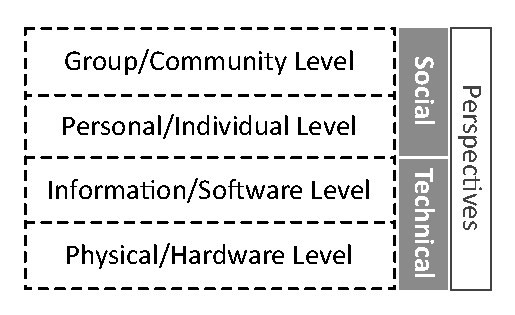
\includegraphics[width=1.0\linewidth]{img/sts_levels.pdf}\\
%	DSO (Distribution System Operators),  SSL (Secure Sockets Layer)
%	\caption{YouPower Platform Overview}\label{fig:platform}
%\end{center}
%\end{figure}

\begin{figure}[t]
\sidecaption[t]
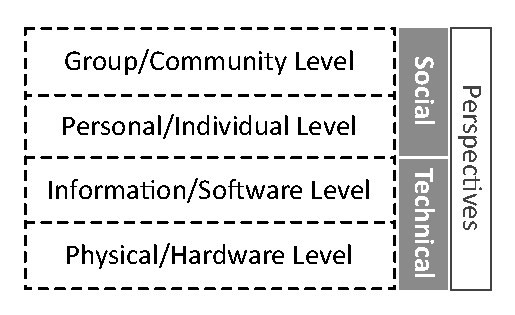
\includegraphics[scale=.65]{img/sts_levels.pdf}
\caption{Levels of socio-technical systems viewing from different perspectives: the levels are not different systems but overlapping views of the same system \cite{Whitworth2009,Whitworth2013}}
\label{fig:sts_levels} 
\end{figure}

Socio-technical systems are systems arising through encompassing people communicating with people whose interactions are mediated (at least partially) by technology rather than the natural world \cite{Whitworth2009}.
The term ``socio-technical'' embodies both a research perspective and a subject matter \cite{Lee2001}. Facing a complex system, researchers from different disciplines often examine the system from their own perspectives. Engineers, for example, see hardware systems, computer scientists see information systems, psychologists see cognitive systems, sociologist see social systems -- in fact, no discipline has a monopoly on science and all those views are valid \cite{Whitworth2013}. 
Figure~\ref{fig:sts_levels} uses the notion of system levels to illustrate this perspective difference in socio-technical systems \cite{Whitworth2009,Whitworth2013}. Notably, the levels in Figure~\ref{fig:sts_levels} are not different systems nor partitions of systems, but overlapping views of the same system corresponding to the engineering, computing, psychological and sociological perspectives \cite{Whitworth2009}. The top and bottom of the levels are open-ended, 
as social groups can coalesce into larger entities such as organizations, cities, nations and beyond \cite{Whitworth2009a}, while physics and hardware can be studied in micro and nano scales. The system boundary and the boundaries of those views are not necessarily clear-cut (hence dawn as dashed lines). A socio-technical systems view is one that incorporates and meaningfully interconnects all levels of considerations: the upper two levels (Group/Community and Personal/Individual) together being social and the lower two (Information/Software and Physical/Hardware) technical. Each upper level can be seen as   ``arising'' or ``emerging'' from the lower levels. For example, personal cognitions ``emerge'' from information exchanges supported by software, which ``arises'' from hardware \cite{Whitworth2009}. The higher a level of view, the higher its degree of abstraction, and the less deterministic and predictive it becomes.  
% 
With the levels of difference perspectives in mind, the socio-technical systems view can be articulated as the recognition of three fundamental properties as follows \cite{Sawyer2014}. 
%
%
\begin{description}
\item[\textit{First, the mutual constitution of people and technologies.}] 
This mutual constitution (by the social and the technological) generates complex and dynamic interactions among technological capacities, social norms, histories, situated context, human choices, actions and so on. In socio-technical systems, social interactions are enabled or supported by technological means. The two adapt to one another, which is referred to as the mutual adaptations. 
%
\item[\textit{Second, the contextual embeddedness of the mutuality.}] 
The context of a sociotechnical system is not taken as static or delineable. There are dynamic situational and temporal conditions that influence 
the mutual adaptations throughout the course of design, development, deployment, uses and even retirement phases of the systems of interest. 
%
\item[\textit{Third, the importance of collective action.}] 
Collective action refers to the joint pursuit of one or more shared (potentially conflicting) goals by two or more interested parties such as problem owners, shareholders, users  and communities affected (without implying positive or negative outcomes). It shapes and is shaped by both the context and the technological components. 
\end{description}
%
%
Researchers who hold a socio-technical systems view investigate more than just the technological (sub-)system or just the social (sub-)system or even the two side by side, but also the phenomena that emerge when the two interact \cite{Lee2001}. A socio-technical approach tries to abstain from oversimplifications that seek a single or dominant cause of change, but studies the complexity, dynamic and uncertainty in the networks of institution, people and technological artefacts in the process of technologically involved change \cite{Sawyer2014}. 
%
The levels of perspectives and the three fundamental properties of socio-technical systems aforementioned help researchers organize, categorize and allocate their inquiries and knowledge. 

What does a socio-technical systems view mean to design in particular? The rest of this section discusses this in three interrelated parts: the impact of a socio-technical systems view
(I) on the understanding of the design problems, (II) on the design process, and (III) on the products or results of the design process.

\runinhead{Understanding the Design Problems or Situation} Designing in socio-technical systems is becoming increasingly challenging partly due to the increasing systems complexity and scale.  
Large-scale socio-technical systems often are not designed as a whole by one team in one project, but are incrementally ``piece by piece'' transformed and evolved from many generations of ``legacy'' systems. Designers and engineers are therefore faced with ill-structured or wicked problems that are not straightforward to determine what systems boundaries to choose, what issues to address and what aspects to consider regarding the design. [BC]

A socio-technical systems view by definition advocates a systemic approach towards understanding including but not limited to information acquisition, diagnosis and analysis. Developing an understanding of the design problems or situation entails firstly looking into the roles, responsibilities, powers, interests and requirements of the stakeholders involved \cite{Checkland1981}. As will be discussed later in the section, iterations in a design process deepens this understanding. 
Pragmatically, a designer can start with upper level (more abstract) views and dive into the lower level (less abstract) ones, i.e. from group/community level towards physical/hardware level as shown in Figure~\ref{fig:sts_levels}.
At each level, the designer investigates questions such as what are the corresponding goals to be achieved (or problems to be tackled) \cite{Checkland1981,Waterson2002} and associated requirements to be fulfilled \cite{Whitworth2009a}, which social/technical elements (or components) are important to each level of views, how do the elements operate/behave individually and interact within and across the levels, and what are the possible outcomes of the interactions and in what context \cite{Baxter2011}. 

Table~\ref{tab:questions} provides a set of such questions categorized by the three socio-technical systems properties and associated to the levels of systems views. The questions are by no means exhaustive but serve as examples to orient ways of thinking during design. 
Given the nature of socio-technical systems, the answers to many of such questions are context specific, influenced by dynamic situational and temporal conditions. \cite{Baxter2011,Norman2015}. This means the contextual information associated with the answers also need to be well studied and documented. 

\begin{table}
\caption{Examples of questions to investigate categorized by socio-technical systems properties and associated to levels of systems views }
\label{tab:questions}       % Give a unique label
%
% Follow this input for your own table layout
%
\begin{tabular}{>{\raggedright}p{2cm}>{\raggedright}p{1.6cm}>{\raggedright}p{1.7cm}p{6.2cm}}
\hline\noalign{\smallskip}
\textbf{Properties}  & \multicolumn{2}{l}{\textbf{Relevant Levels of Views}} &   \textbf{Examples of Questions to Investigate} \\
  &   \textit{Most relevant} & \textit{Can be relevant} &  \\
\noalign{\smallskip}\svhline\noalign{\smallskip}
Mutual & All & -- & Which elements (or components) are important? $^a$  \\
constitution &   &  & How do the elements behave and interact?\\
  &   &  & What are the possible outcomes of the interactios?\\
  &   &  & What are the goals, constrains and requirements, if any, of the elements?\\ \hline\noalign{\smallskip}
Contextual embeddedness &   Group/ community &  Information/ software & What are the situational and temporal conditions with which behaviours and interactions take place? \\
 &   Personal/ individual &  Physical/ hardware & What are the influences of  the situational and temporal conditions on the outcomes of the behaviours and interactions?\\
 &     &    & How those situational conditions may change over time?\\ \hline\noalign{\smallskip}
Collective action   & Group/ community  &  Information/ software & What are the community (or institutional) goals, constrains and requirements?\\
   &  Personal/ individual  & Physical/ hardware & How are the community (or institutional) goals, constrains and requirements aligned with the individual goals, constrains and requirements? \\
   &&& What is the group and individual attitude towards the community (or institutional) goals or collective action? \\ \hline\noalign{\smallskip}
General $^b$ & All  &  --  & What is the level of resolution to use when describing and analysing the system? \\
&&& What is the set of values that underpin the design thinking about the system? \\
&&& What are the criteria and metric of evaluating if and to what degree the desired goals are achieved and maintained? \\
\noalign{\smallskip}\hline\noalign{\smallskip}
\end{tabular}
$^a$ Elements can also be weighted in scale, e.g. from \textit{important} (must be included in the study), to \textit{can be relevant} (can be included in the study), to \textit{least important} (can be excluded from the study).\\
$^b$ It concerns all three properties above. 
\end{table}



\begin{figure}
\sidecaption
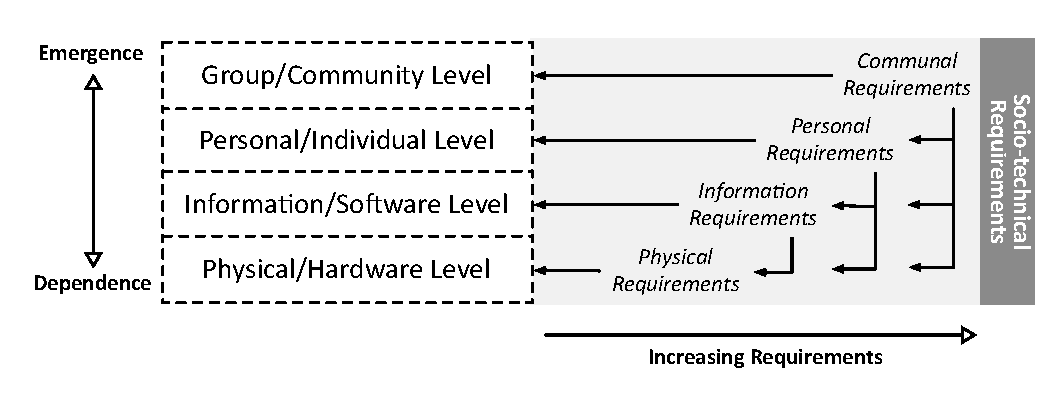
\includegraphics[scale=.66]{img/sts_requirements.pdf}
\caption{Levels of socio-technical requirements \cite{Whitworth2009a}}}
\label{fig:sts_requirements} 
\end{figure}

In a socio-technical approach, social requirements must become part of technical design \cite{Whitworth2014}. This is well illustrated in Figure~\ref{fig:sts_requirements} \cite{Whitworth2009a}.


A ``social-technical  gap''  emerges when there is a  deficit  between  what  society  needs  and  what technology does \cite{Whitworth2014}. 

\begin{svgraybox}

\runinhead{Design Process} The design process of socio-technical systems can be seen as a decision-making process where the problem owners, shareholders, users, etc. participate to represent their interests. Often, the design porcess is so complex that the process itself can be deemed as a socio-technical system \cite{Baxter2011}. 



Designers are therefore working \textit{in} the context of some socio-technical system with the intention of changing or improving some part of that system [BC]. 

It is often conceived and implemented in participatory decision-making processes actively involving stakeholders

\runinhead{Products or Results of the Design Process}
kln





\runinhead{Products of the design process} these not only consists of technological artifacts but also may include rules for behaviour, policies, etc. through which the designer wish to intervene in social-technical systems. what is it that we are designing? 

\runinhead{Design process} The design process can be seen as a decision-making process where the problem owners, shareholders, users, etc. participate to represent their interests. It is often conceived and implemented in participatory decision-making processes actively involving stakeholders



The evolutionary nature of large-scale socio-technical systems means that what matters more in the design is the design process itself, more than the ``final status'' of the system \cite{Shin2014, need more ref} because the socio-technical system keeps evolving and exhibits emergent behaviour \cite{Nikolic2009}. An important  goal of the design process is to make the design (a product or system) relevant to the evolving context \cite{Shin2014, need more ref} as social and technical artifacts exist within their socio-technical context [BC]. 

\end{svgraybox}



\begin{svgraybox}
can be put in the discussion: 
acontextual and detemporalized perspective approaches , general solution ., is self-limiting 
focus on situating work and seek to examine all contextual factors , this types of inquiry attempt to construct a holistic view of context: one that does not diminish or remove contextual elements, even those with limited influence. 
paying little attention to the environment of the organization and temporal dimension of technological innovation  \cite{Sawyer2014}
\end{svgraybox}


\begin{svgraybox}
Use and combine content in: (the literature can be connected, e.g. problems mentioned in Norman and Baxter  can be mapped to the four layers in Whitworth )
\begin{enumerate}
\item \cite{Norman2015} (design problems in large-scale socio-technical systems) and 
\item \cite{Baxter2011} (socio-technical approach to systems engineering)
\item \cite{Whitworth2009} (four system levels of Socio-tehnical systems); 
\item \cite{Shin2014} (a very good article about IoT, socio-technical perspective )
\item see also https://medium.com/rettigs-notes/notes-on-sociotechnical-systems-design-178f161bc9e8 
\end{enumerate}
\end{svgraybox}

